\documentclass{article}
\usepackage{graphicx} % Required for inserting images
\usepackage{amsmath} 
\usepackage{amssymb}
\usepackage{xcolor}
\usepackage{hyperref}
\usepackage[margin=1.2in]{geometry}

\title{The Finite Element Method applied to Selected Differential Equations}

\author{Patryk Drozd and Adriana Voloshyna }
\date{2024}

\begin{document}

\maketitle

\section{Background}
There is no doubt that differential equations are ubiquitous in all of physics, and yet often times they can be difficult to solve analytically. Scientists and engineers therefore turn to computational methods in hopes of finding solutions to the differential equations which govern the most fundamental laws of physics. For example, one such set of differential equations are the Navier-Stokes equations, which remain the most reliable tool in understanding the motion of fluids. Despite the widespread practicality of these equations, there is still much to be studied about them. In fact it has not been proven that these equations always have smooth (i.e. infinitely differentiable) solutions in three dimensions. This conundrum is of great interest to the mathematical community, and is one of the seven Millenium Prize Problems, meaning that the Clay Mathematics Institute has offered a prize of one million US dollars for the first correct proof of existence and smoothness or a counterexample. Inspired by the mystery of these equations, we set out to investigate this intriguing world of differential equations using a particular algorithm known as the Finite Element Method (FEM). 


\section{Introduction}
The aim of this project is to solve a number of ordinary and partial differential equations using FEM. To do this, we must begin by studying the mathematical background of the method. A significant portion of this report will focus on the derivation of the necessary tools needed to justify the credibility of this method. A walk-through of the implementation of the method for specific problems will also be provided, alongside results that we obtain from solving these problems. 
\subsection{Computational Methods}
Before choosing our method of computation, we investigated the strengths and weaknesses of several computational methods, such as the Finite Volume Method, Finite Difference Method, and the Finite Element Method.

The Finite Volume Method involves subdividing a space (or volume) into a finite number of cells, creating a discretised collection of what are known as control volumes. Given a partial differential equation which can be written in divergence form, we can use Gauss' Divergence Theorem to rewrite a volume integral into a surface integral, and calculate the flux at each of the surfaces of the cells. This method relies on the conservation of flux, i.e. that the outward flux in each cell must be equal in magnitude to the inward flux entering the cell.

The Finite Difference Method is the most straightforward way to numerically solve a system of differential equations. The domain is discretised into a finite set nodal points, and the derivatives in question are approximated using finite difference (usually a central finite difference). This just means that we take the definition of a derivative from First Principles, but instead of finding the limit as the differential (the small change in x) goes to zero, we give it a very small but non-zero value. Then, for each nodal point we can find the value of a solution at that point, which together gives a numerical solution to a given system of differential equations. This method is efficient in computing solutions on a rectangular domain, but it is difficult to implement on an irregularly shaped domain.

The Finite Element Method also begins with discretising a domain into a finite number of elements. These elements are geometric shapes which together create a mesh for the given domain. To obtain a solution, a set of differential equations together with boundary conditions must first be expressed in what is known as the weak formulation. Then, for a given set of basis functions, we can find a solution for each element of the mesh and together this gives a solution to the system. This method is more mathematically involved than the others and has the least limitations on what type of equations or domains it can be used for. We thus decided that this method would not only be best suited to finding solutions to various types of differential equations, but also would be interesting to study from a more mathematical perspective. 
\subsection{Background of the Finite Element Method} 
The Finite Element Method is a popular numerical method of solving differential equations. It can accurately approximate a solution to a boundary value problem when analytic solutions are difficult or impossible to find. Using this method we can model and study physical phenomena such as heat transfer, structural behaviour, fluid flow and electromagnetic potential. Finite Element Analysis is often used in engineering as it can accurately replicate simulations of different types of conditions in a cost effective, safe and efficient way. A very early example of this was NASTRAN, an open source Finite Element Analysis program developed for NASA in the 1960s to aid engineers in structural analysis. The program was so successful that it is still used in aerospace, maritime and automotive industries across the globe today. 


\section{One Dimensional Poisson Problem}
To gain an understanding of the algorithm behind the Finite Element Method, we begin by solving the one dimensional Poisson problem. This problem is an easy differential equation to begin our investigation with, and has many physical applications, such as in finding magnetic or electric potential due to charge or current distributions. \\
Thus we want to find solutions \textit{u} which satisfy the differential equation

\[-\nabla^{2}u = f  \qquad\textrm{on domain }\Omega \]
with the boundary condition 

\[u = 0 \qquad\textrm{on } \partial\Omega\]
Note that in the one dimensional case, the Laplacian $\nabla^{2}$ is simply the second derivative of u. Taking the domain to be the interval [0,1], the differential equation reduces to 

$$ -u'' = f \qquad\textrm{on }[0,1] $$
and the boundary condition can be written as
$$ u(0) = u(1) = 0. $$

The above is what is known as the strong formulation of the Poisson problem. We can express this alternatively using the weak formulation.
\subsection{Derivation of the Weak Formulation}
The weak formulation of the one dimensional Poisson problem can be described as follows:\\
\\
Given a function space 
$$ V := \{v| \textrm{ $v$ is continuous on [0,1], $v'$ is piecewise continuous and bounded on } [0,1],  v(0) = v(1) = 0 \} $$
we must find a $u$ $\epsilon$ $V$ such that 
\[(u',\phi ') = (f , \phi) \qquad\forall\,\phi\, \epsilon\, V\]
where 
$(u,v) := \int_{0}^{1} u(x)v(x) \,dx $
is the scalar product of functions u and v on [0,1].\\
\\
To see that these formulations are equivalent, observe that if $-u'' = f$, we can multiply both sides by a test function $\phi$ and integrate over our domain to obtain 
\[-\int_{0}^{1} u''(x)\phi(x) \,dx = \int_{0}^{1} f(x)\phi(x) \,dx \qquad\forall\,\phi\, \epsilon\, V\]
after which we can use integration by parts to rewrite this as
\[- ( [u'(x)\phi(x)]_0^1 - \int_{0}^{1} u'(x)\phi'(x) \,dx ) = \]
\[\int_{0}^{1} u'(x)\phi'(x) \,dx - [ u'(1)\phi(1) - u'(0)\phi(0) ] = \int_{0}^{1} f(x)\phi(x) \,dx
\qquad\forall\,\phi\, \epsilon\, V. \]
But since $\phi$ $\epsilon$ $V$ , it must satisfy the boundary conditions $\phi(0)$ = $\phi(1)$ = 0, which causes the above to reduce to
\[\int_{0}^{1} u'(x)\phi'(x) \,dx  = \int_{0}^{1} f(x)\phi(x) \,dx \qquad\forall\,\phi\, \epsilon\, V \qquad\textrm{ as required.}\] 
\\
\\
To show implication in the other direction, and therefore proving equivalence, we repeat the steps above in the reverse direction. Let 
\[(u',\phi ') = (f , \phi) \qquad\forall\,\phi\, \epsilon\, V  \]
and take away 0 from the left side of the equation by using the boundary conditions which $\phi$ must satisfy
\[(u',\phi ') - [u'(1)\phi(1) - u'(0)\phi(0)] = (f , \phi) \qquad\forall\,\phi\, \epsilon\, V.  \]
We observe that the above can be reduced to 
\[(-u'',\phi ) = (f , \phi) \]
which can be rewritten as 
\[(-u'',\phi ) - (f , \phi) = (u'' - f,\phi )   = 0 \]
Since this must hold $\forall\,\phi\, \epsilon\, V$, we can conclude that
\[-u'' - f = 0 \qquad \textrm{on }[0,1]\]
and so we have that the strong and weak form are equivalent. 
\subsection{Discretisation of the the Function Space}
Since computers of our age are not comfortable with infinities, we must discretise the infinite dimensional function space $V$, into a finite dimensional subspace $V_h$. To do so, we must create a mesh on which we will use basis functions to approximate a solution to our problem. This mesh provides a way of dividing our continuous domain, in this case the interval [0,1], into a finite amount of nodal points (or vertices) $x_i$ with 
$x_0 = 0$,..., $x_{n} = 1$.

On the interval between each nodal point $(x_i, x_{i+1})$, we can define a \textbf{Finite Element} $(K, P, \Sigma)$  where \\
- K is a cell of the mesh, also called an element \\
- P are polynomials on K and \\
- $\Sigma$ is a set of degrees of freedom. \\
Note that for this problem we will be working only with $\Sigma$ = 1, as our basis functions will be linear. If, for example, we wanted to use quadratic polynomials as our basis functions, we would set $\Sigma$ = 2, but for the purpose of solving the one dimensional Poisson problem, this would add an unnecessary degree of complexity. \\
\\
Now we have the tools to construct our finite dimensional subspace,
$$ V_h := \{v| \textrm{ $v$ is continuous on [0,1], } v|_{K_i}\, \epsilon\, P \textrm{ for each } i,\,  v(0) = v(1) = 0 \}. $$

\subsection{Basis Functions}
  The basis functions $\phi_i$ are simple polynomials which can be used to describe an element of our finite dimensional subspace $V_h$. A function $v$ has a unique representation in $V_h$ given by 
 $v_h(x) = \sum_{i=0}^{n}v_i\phi_i(x)$ where $n$ is the amount of nodal points in our interval, as before. Each basis function will be scaled by a constant $v_i$, and must satisfy $$\phi_i(x_j) =  \begin{cases} 
      1 & i = j \\
      0 & i \neq j.
   \end{cases}$$
Say for example we want to construct a function $v_h(x) = 1\cdot \phi_{0.25}(x) + 1\cdot \phi_{0.5}(x) + 1\cdot \phi_{0.75}(x)$. The figure on the left shows how the sum of the individual (scaled) bases superimpose to form our function. 
Similarly we can scale the basis functions to construct a function $v_h(x) = 1\cdot \phi_{0.25}(x) + 3\cdot \phi_{0.5}(x) + 2\cdot \phi_{0.75}(x)$, as can be seen on the right figure.
\begin{figure}[hbt!]
\centering
\begin{minipage}{.5\textwidth}
    \centering
    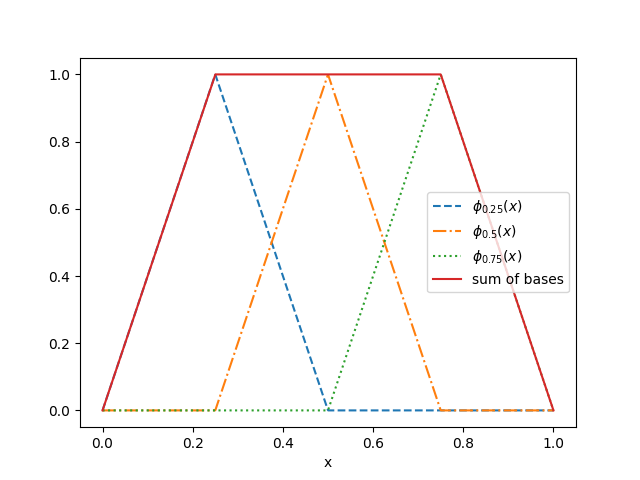
\includegraphics[width=8cm]{basis functions/linear_basis_sum.png}
    \caption{Sum of linear bases}
    \label{fig:Sum of linear bases}

\end{minipage}%
\begin{minipage}{.5\textwidth}
    \centering
    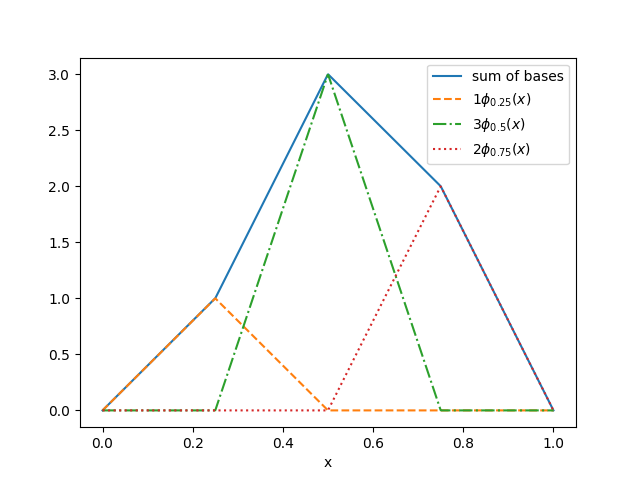
\includegraphics[width=8cm]{basis functions/linear_basis_sum_funky.png}
    \caption{Sum of scaled linear bases}
    \label{fig:Sum of linear bases}

\end{minipage}
\end{figure}
\subsection{Discretisation of the Weak Formulation}
The weak form of the Poisson problem can now be discretised to the following:
For a function space $V_h$ (as described previously), we must find a $u_h$ $\epsilon$ $V_h$ such that 
\[(u_h',\phi_h ') = (f , \phi_h) \qquad\forall\,\phi_h\, \epsilon\, V_h.\]
We can write $u_h'$ in terms of its basis functions to obtain:
\[((\sum_{j=0}^{n}u_j\phi_j'),\phi_h ') = (f , \phi_h) \qquad\forall\,\phi_h\, \epsilon\, V_h.\]
Furthermore, since any function $\phi_h$ can be written as a linear composition of basis functions, it is enough to show that
\[((\sum_{j=0}^{n}u_j\phi_j)',\phi_i ') = (f , \phi_i) \qquad\forall\,0 \leq i \leq n\]
\[\iff \sum_{j=0}^{n}u_j(\phi_j',\phi_i ') = (f , \phi_i) \qquad\forall\,0 \leq i \leq n. \]
Now we search for a sequence of constants $(u_j)$ which satisfy the equivalence above. 
\subsection{Linear System Representation}
To do this computationally, we can represent the linear system in the form of a matrix equation
\[\begin{pmatrix}
(\phi_1',\phi_1 ') & (\phi_1',\phi_2 ') & \hdots &(\phi_1',\phi_n ')\\
(\phi_2',\phi_1 ') & (\phi_2',\phi_2 ') & \hdots &(\phi_2',\phi_n ')\\
\vdots &  \vdots &  \ddots &  \vdots\\
(\phi_n',\phi_1 ') & (\phi_n',\phi_2 ') &\hdots &(\phi_n',\phi_n ')
\end{pmatrix}
\begin{pmatrix}
u_1\\
u_2\\
\vdots\\
u_n
\end{pmatrix} =
\begin{pmatrix}
(f , \phi_1) \\
(f , \phi_2) \\
\vdots\\
(f , \phi_n)
\end{pmatrix}\]
to find a vector $\vec{u}\ \epsilon\ \mathbb{R}^n$ which satisfies this equation. For clarity, let us rewrite the above equation as $$A \vec{u} = F$$ Solving a linear system like this is not difficult - we simply multiply both sides of the equation with the inverse of $A$ to obtain what $\vec{u}$ is equal to. All that remains is to find the components of $A$, i.e. the scalar product of the basis functions. 
\subsection{Matrix $A$}
Due to the symmetry of the matrix, we begin by solving the diagonal elements, which are all of the form $(\phi_i',\phi_i')$. Lets take a look at one basis function $\phi_i$ which is non-zero only on the interval $[x_{i-1}$, $x_{i+1}]$. If h is the distance from $x_{i-1}$ to $x_{i}$ and the height of the basis function is set to 1, then $$\phi_i(x) = \frac{x}{h}\qquad \textrm{when restricted to the interval} \qquad[x_{i-1}, x_{i}].$$ By symmetry, $$\phi_i(x) = 1 - \frac{x}{h} \qquad \textrm{on the interval}\qquad [x_{i}, x_{i+1}].$$  Then 
$$\int_{0}^{1} \phi_i'(x)\phi_i'(x) \,dx = \int_{x_{i-1}}^{x_{i+1}} \phi_i'(x)\phi_i'(x) \,dx = \int_{x_{i-1}}^{x_{i}} \left(\frac{1}{h}\right)\left(\frac{1}{h}\right)\,dx\, + \int_{x_{i}}^{x_{i+1}} \left(-\frac{1}{h}\right)\left(-\frac{1}{h}\right) \,dx $$ 
$$= \left[\frac{x}{h^2}\right]_{x_{i-1}}^{x_{i}} + \left[\frac{x}{h^2}\right]_{x_{i}}^{x_{i+1}} = \frac{h}{h^2} + \frac{h}{h^2} = \frac{2}{h}.$$ 
Now to find the elements next to the diagonal, we must calculate $(\phi_i',\phi_{i+1}')$ = $(\phi_{i+1}',\phi_i')$. Since $\phi_i = 0$ anywhere outside the interval $[x_{i-1}$, $x_{i+1}]$, we can limit our integral to the same interval. Moreover, $\phi_i+1 = 0$ on the interval $[x_{i-1}$, $x_{i}]$, so we can further restrict our limits of integration to $x_{i}$ and $x_{i+1}$. 
$$\int_{x_{i}}^{x_{i+1}} \phi_i'(x)\phi_{i+1}'(x) \,dx = \int_{x_{i}}^{x_{i+1}} \left(-\frac{1}{h}\right)\left(\frac{1}{h}\right)\,dx  = \left[-\frac{x}{h^2}\right]_{x_{i}}^{x_{i+1}} = -\frac{1}{h}.$$ 
Finally observe that any matrix elements other than those which we have calculated must equal to zero, as the two basis functions in the scalar product will never be non-zero on the same interval. This gives us a sparse matrix, one in which only a small number of entries are non-zero, which can save a lot of memory and storage space when searching for solutions to our linear system. This matrix is also clearly symmetric. This comes from the fact that basis elements commute, i.e. $\phi_i \phi_j = \phi_j \phi_i$.
\subsection{Matrix $F$}
To begin solving the left hand side of the equation, we must chose a function $f$. For the sake of simplicity, let $f = 1$. Then, for any basis function $\phi_i(x)$, $$(f , \phi_i) = \int_{0}^{1} f(x)\phi_i(x) \,dx  = (1) \int_{x_{i-1}}^{x_{i+1}} \phi_i(x) \,dx =  \int_{x_{i-1}}^{x_{i}} \left(\frac{x}{h}\right)\,dx\, + \int_{x_{i}}^{x_{i+1}} \left(1 -\frac{x}{h}\right) \,dx =  h.$$ 
\\
\subsection{Numerical Implementation and Solution}
\begin{figure}[hbt!]
\centering
\begin{minipage}{.5\textwidth}
    \centering
    \includegraphics[width=8cm]{poisson 1d/(Poisson_1d)_(lin_matrix_A)_(x)_(vertex_num_9).png}
    \caption{Matrix A for 9 nodal points}
    \label{fig:Matrix A for 9 nodal points}

\end{minipage}%
\begin{minipage}{.5\textwidth}
    \centering
    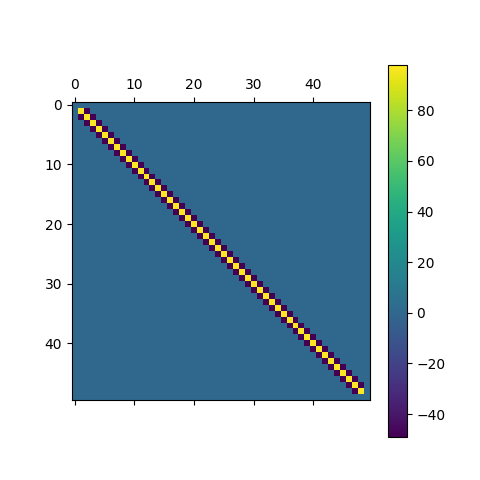
\includegraphics[width=8cm]{poisson 1d/(Poisson_1d)_(lin_matrix_A)_(x)_(vertex_num_50).png}
    \caption{Matrix A for 50 nodal points}
    \label{fig:Matrix A for 50 nodal points}

\end{minipage}
\end{figure}
Although it is possible to solve the scalar products of basis functions analytically, it can become tedious for large mesh sizes and non linear basis functions. Using the trapezoidal integration function (np.trapz), we can solve for the elements of the matrix numerically. To see that this numerical method can reproduce the same results that we achieved analytically, we plotted the elements of the matrix $A$. Observe in the figure above the results for a system with 9 nodal points and a system with 50 nodal points. Indeed we get a sparse matrix with non-zero elements only along the diagonal and one above or below the diagonal. 
\\
\\
Now that we have a linear system $A \vec{u} = F$, and the tools to obtain this equation numerically, we can look for solutions $\vec{u}$. To do this, it is necessary to create three nested for loops. For each element of our mesh, we find the scalar product of our function $f$ with our basis functions $\phi_i$ for all $i$. Then, for each basis function $\phi_i$, we take the scalar product of $\phi_i$ and $\phi_j$, for all $j$, which gives us a row of the matrix $A$ for each iteration of $i$. Using numpy.linalg.pinv we find the inverse of this matrix, and thus solve for $\vec{u}$. We are now ready to plot $\vec{u}$ to see the solutions to the one dimensional Poisson problem. Note how the curve is smoother when we consider a finer mesh with more nodal points. 
\begin{figure}[hbt!]
\centering
\begin{minipage}{.5\textwidth}
    \centering
    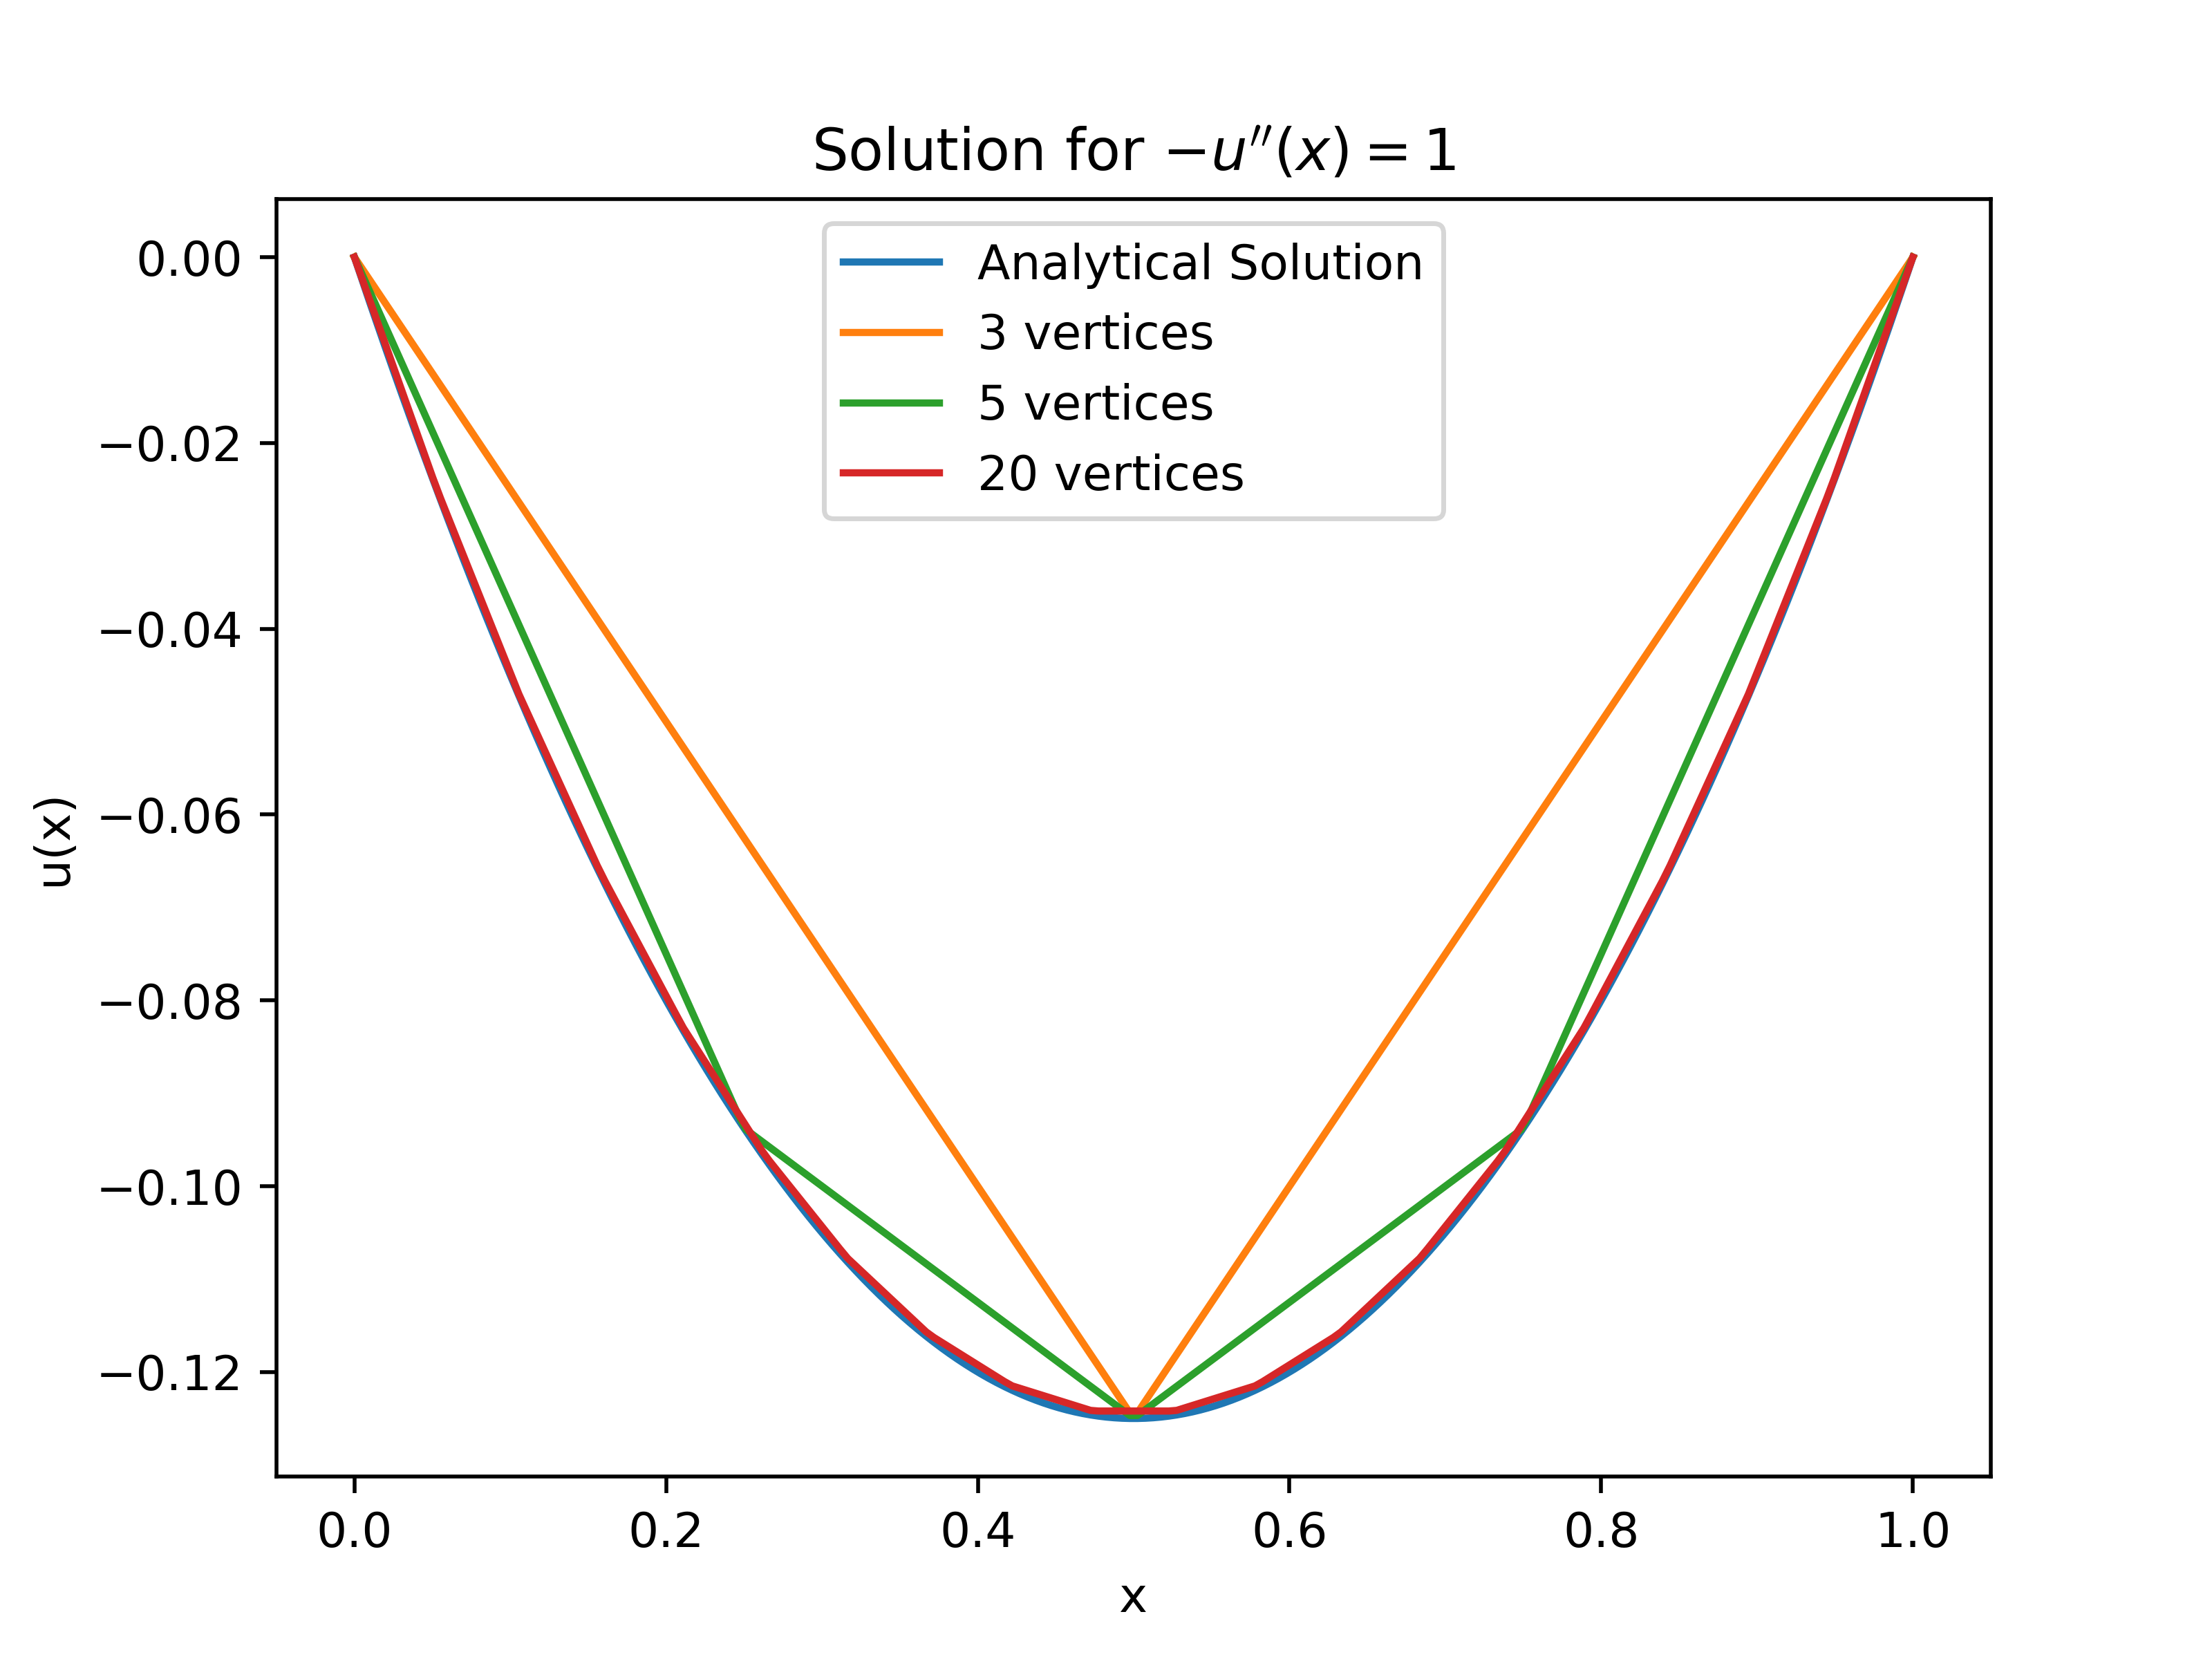
\includegraphics[width=8cm]{poisson 1d/(Poisson_1d)_(lin_sol).png}
    \caption{Solutions for various mesh sizes}
    \label{fig:Solution for given nodal points}

\end{minipage}%
\begin{minipage}{.5\textwidth}
    \centering
    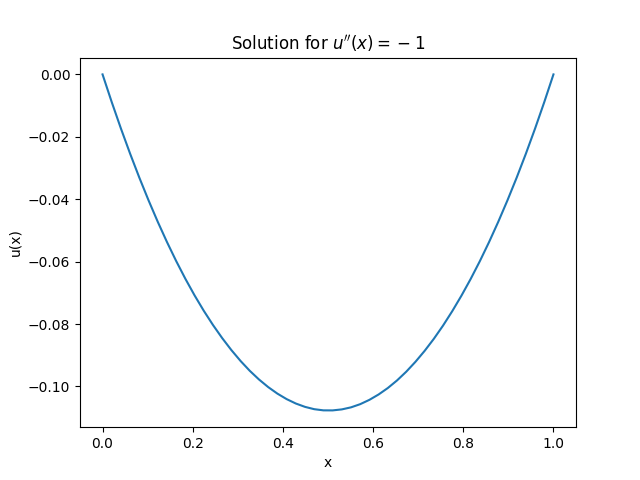
\includegraphics[width=8cm]{poisson 1d/(Poisson_1d)_(lin_sol)_(vertex_num_50).png}
    \caption{Solution for 50 nodal points}
    \label{fig:Solution for 50 nodal points}

\end{minipage}
\end{figure}
\\
\\
\\
If we choose $f = x$, we obtain the following solution for $\vec{u}$:
\begin{figure}[hbt!]
    \centering
    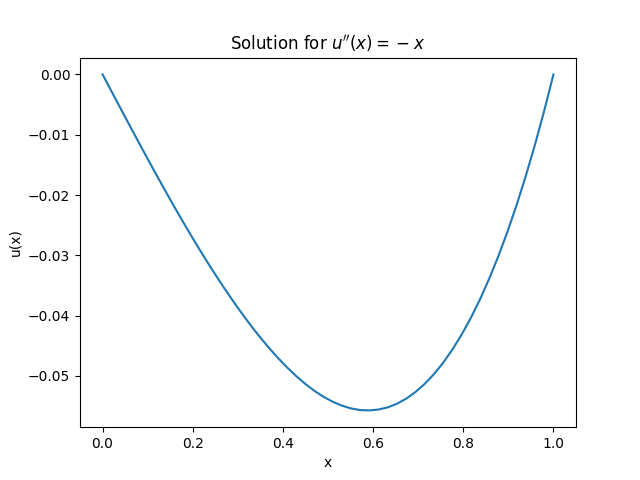
\includegraphics[width=8cm]{poisson 1d/(Poisson_1d)_(lin_sol)_(x)_(vertex_num_50).png}
    \caption{Solution for 50 nodal points}
    \label{fig:linear basis sum}
\end{figure}
\\
To check that our solutions are correct, we compare our numerical results to the analytic solutions of these equations. Using our knowledge of second-order linear ordinary differential equations, we obtain the analytic solutions  $$u(x) = \frac{1}{2} x(x - 1)  \qquad \textrm{for} \quad f(x) = 1,$$ 
$$u(x) = \frac{1}{6} x(x^2 - 1) \qquad \textrm{for} \quad f(x) = x.$$
Plotting these functions (on Wolfram Alpha) we can see that for a sufficient number of nodal points $n$ our numerical solutions are an accurate approximation of the analytic solutions.

\section{Two Dimensional Poisson Problem}
To solve the two dimensional Poisson problem, we wish to find a function $u(x,y)$ which satisfies 
\[\nabla^{2}u = f\,\,\textrm{on }\Omega \quad \textrm{with mixed Neumann and Dirichlet boundary conditions}.\]
Here the domain is a unit length square $[0,1]\times[0,1]$, and the Laplacian $\nabla^{2} =$ {\large$\frac{\partial^2}{\partial x^2}$} $+$ {\large$\frac{\partial^2}{\partial y^2}$}. We decided to experiment with the types of boundary conditions which we can impose. The motivation behind this was the idea that often in physics we have a fluid which flows in from one end of a "box", i.e. we enforce that our solution has a non zero derivative on one side of our domain, and it dissipates on the remaining boundaries of the domain. We therefore impose Neumann boundary conditions (boundary conditions on the directional derivative of $u$ as opposed to $u$ itself)  of the form $$\nabla u(x,y)\cdot \hat{n} = -x(x-1) \qquad \forall\, (x,y)\, \epsilon \,\partial\Omega_N \subset \partial\Omega,$$
and the Dirichlet boundary conditions are $u(x,y) = 0 \, \textrm{on } \,\partial\Omega_D\subset\partial\Omega$
 and we choose $$\partial\Omega_N = \{1\}\times [0,1] \quad \textrm{and} \quad \partial\Omega_D = (\{0\}\times [0,1]) \cup ([0,1]\times\{0\})\cup ([0,1]\times\{1\}). $$
The two dimensional Poisson problem can also be written in its weak formulation. To do this, we must first define an infinite dimensional function space:
$$V := \{v(x,y)| \,v, \nabla v \,\epsilon\, L^2(\Omega),  v = 0 \,\, \textrm{on } \partial\Omega_D\}.$$
Here $L^2(\Omega)$ is a space of functions which are square integrable on the given domain. The reason we need to introduce a slightly complicated function space, is to ensure uniqueness of a solution. When we proceed to search for solutions on our mesh, we could encounter problems of uniqueness of a function at the boundary of each cell. But since a line has Lebesgue Measure zero (meaning that a line in the real plane does not contribute to the value of an integral), we can surpass this problem by defining functions to be in a sense equal if they have the same "size", i.e. they are equal in their $L^2$ norm. In this test space, we only restrict our functions with the Dirichlet boundary condition and not the Neumann boundary condition. The latter will appear in the weak formulation of the problem. 

\subsection{The Weak Formulation}
Now we can find the weak formulation of the Poisson problem in the same way as we did previously. We multiply both sides of the equation by a test function $\phi(x,y)$ and integrate both sides over the entire domain. Then using integration by parts (in particular an application of Green's first identity) and applying the Dirichlet boundary condition we obtain
\[\int_{\Omega} \nabla^2 u \,\phi \,dxdy = - \int_{\Omega} \nabla u\cdot\nabla\phi \,dxdy + \int_{\partial\Omega} \nabla u\cdot \hat{n} \,\phi \,dxdy
= \int_{\Omega} f(x,y)\phi(x,y) \,\,dxdy \qquad\forall\,\phi\, \epsilon\, V.\]
Implementing the Neumann boundary conditions gives
$$\int_{\Omega} \nabla u\cdot\nabla\phi \,dxdy =
 - \int_{\Omega} f\phi \,\,dxdy - \int_{\partial\Omega_N}x(x-1) \,\phi \,dxdy\qquad\forall\,\phi\, \epsilon\, V.$$

\subsection{Basis Functions and Discretisation}
We once again only consider a discretised subspace of $V$, namely $V_h$ where we restrict each $v_h$ $\epsilon$ $V_h$ to be polynomial on each element of our mesh. We similarly define basis functions $\phi_i$ to describe the functions in our discretised subspace, except this time the basis functions must describe two dimensional functions. This is done by subdividing the square $[0,1]\times[0,1]$ into  a grid of $n\times n$ smaller squares. On each such square, we want a basis function to be 1 on one corner of the square and 0 on the other three. This can be achieved by taking the product of a basis function on the x-axis with a similar basis function on the y-axis. Letting h be the length of each interval (and therefore also the side length of each square) we get that $$ \phi_{a,b}(x,y) = \phi_a(x)\cdot\phi_b(y)  = \frac{xy}{h^2}.$$
But we also want the neighbouring three squares to peak at the same point, i.e. we want to create an almost pyramidal shape across four adjacent squares. So we define 
$$\phi_{i}(x,y) =  \begin{cases} 
      \phi_{00}(x,y) = \frac{xy}{h^2} & x\,\epsilon\, (x_{i-1}, x_{i}),\, \,y\,\epsilon\, (y_{i-1}, y_{i})\\
      \phi_{01}(x,y) = \frac{x}{h}(1 - \frac{y}{h})& x \,\epsilon\, (x_{i-1}, x_{i}), \,\,y\,\epsilon\, (y_{i}, y_{i+1})\\
      \phi_{10}(x,y) = (1 - \frac{x}{h})\frac{y}{h} & x \,\epsilon\, (x_{i}, x_{i+1}), \,\,y\,\epsilon\, (y_{i-1}, y_{i}) \\
      \phi_{11}(x,y) = (1 - \frac{x}{h})(1 - \frac{y}{h})& x\,\epsilon\, (x_{i}, x_{i+1}),\,\,y\,\epsilon\, (y_{i}, y_{i+1})\\
      0 & \textrm{elsewhere}
   \end{cases}$$
where $i$ denotes where the peak of this basis function will be. The basis functions are linear on x and y, and still polynomial on each element of our mesh. Observe below what one such basis function looks like. 
\begin{figure}[hbt!]
    \centering
    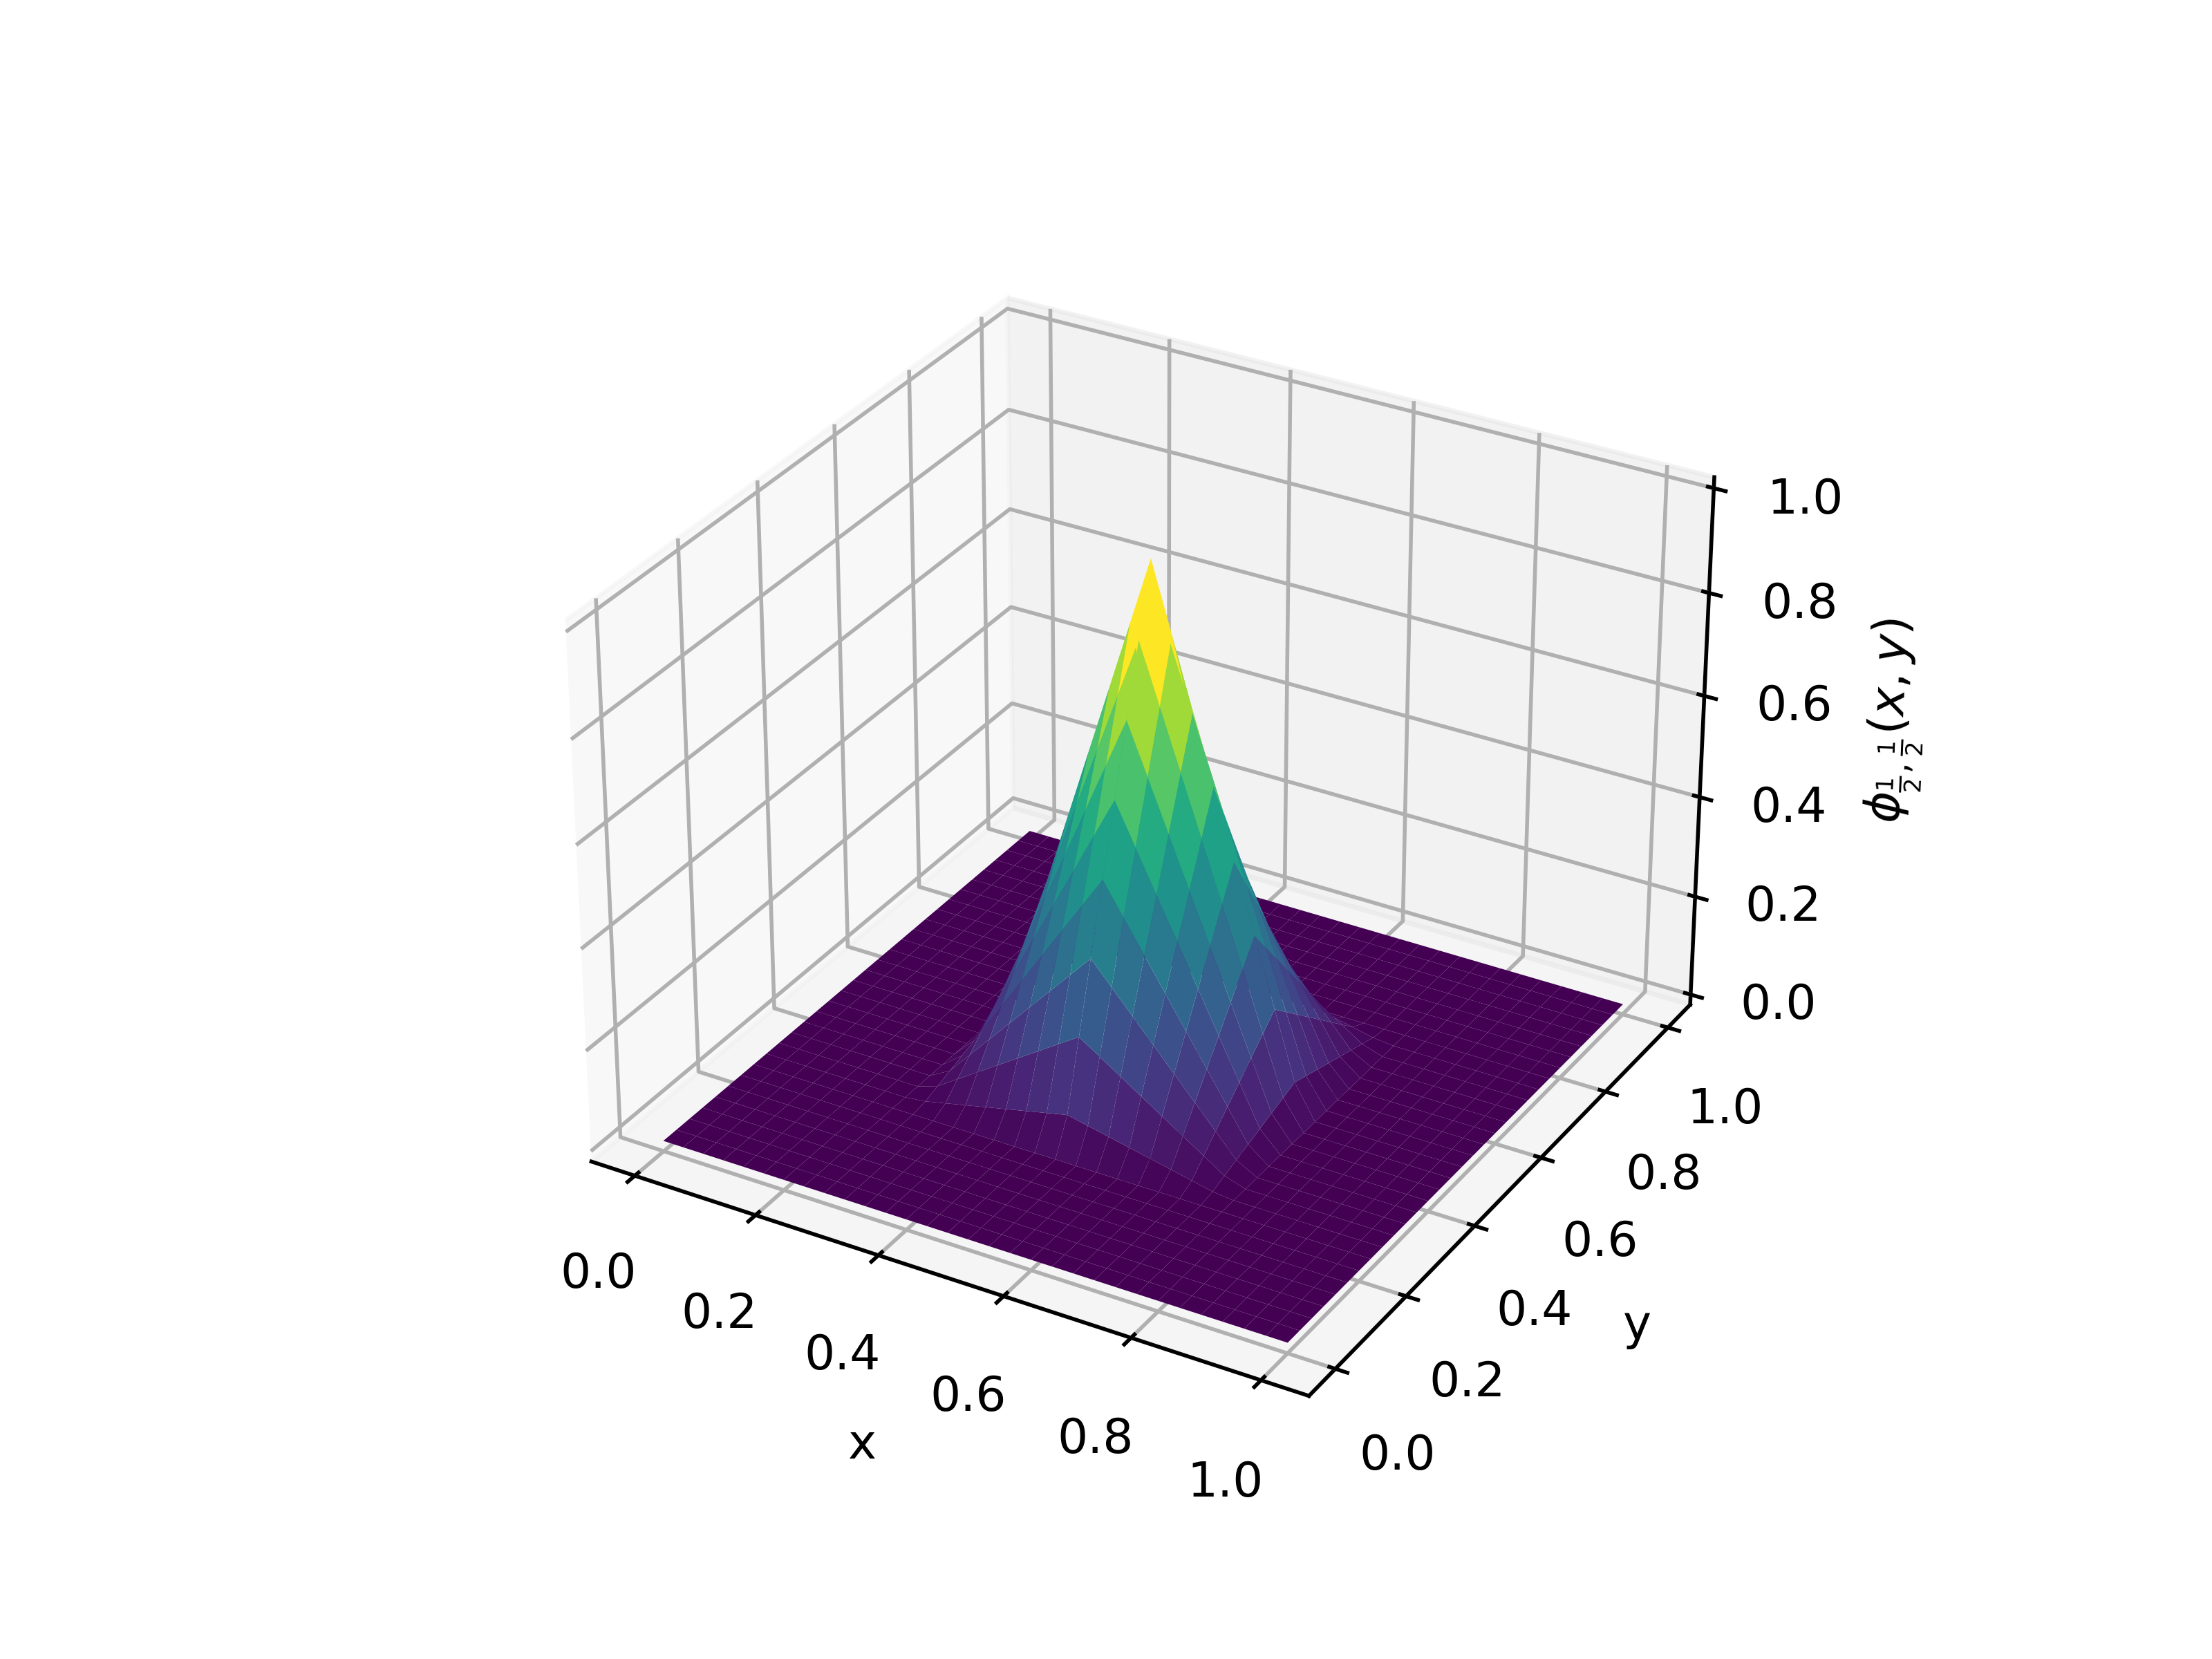
\includegraphics[width=13cm]{basis functions/hat_basis_2d.png}
    \caption{Two Dimensional Basis Function}
    \label{fig:basis}
\end{figure}
\\
\\
We now begin to assemble our problem as we did before into a linear matrix equation. The function $u(x,y)$ can be written as $u_h(x,y) = \sum_{i=0}^{n}u_i\phi_i(x,y)$, and similarly the test function $\phi$ can be replaced with a basis function $\phi_i(x,y)$ and summed over all $0 \leq i \leq n.$ The problem is expressed in the form $$A \vec{u} = F,$$ where $\vec{u}$ is the same as for the one dimensional case, just a sequence of constants which will be our solution. Matrix $A$ (of size $i\times j$) will have elements of the form $$\int_{\Omega} \nabla \phi_i \cdot\nabla\phi_j \,dxdy.$$
Note also that while the gradient of a scalar would give us a vector, we immediately dot product it with another vector (giving us back a scalar), so no complications arise in terms of having to do vector integration. The integration part of the problem we done simply using two np.trapz functions.\\
\\
Matrix $F$ (of size $j\times 1$) has elements of the form
$$- \int_{\Omega} f(x,y)\phi_j \,\,dxdy - x(x-1)\int_{\partial\Omega_N} \,\phi_j \,dy.$$
Recall that the second integral above is calculated only on the line $\{1\}\times [0,1]$, hence why we can treat it as a line integral in the y direction. 
\subsection{Implementation and Results}
The implementation procedure is similar to what was done for the 1 dimensional case. It is interesting to note that in most popular libraries which provide easy interface to use FEM, the meshes have somewhat randomly placed nodes and triangular elements. For the 1 dimensional and 2 dimensional problems, we decided to use square elements because of the ease of implementation. Triangular elements and their associated nodes would have a different set of basis functions and the integrals needed for the weak formulation of the equations would need to be evaluated over triangular domains. On the other hand square meshes only need 2 arrays to be defined. Each basis function will only need to be shifted according to the position of the node and the integrals will be very easy to visualise as they are on square domains. It also means that the implementation for the 2 dimensional case can be relatively easily adapted from the 1 dimensional case. \\
\\
Another key difference in implementation with respect to the one dimensional case is the way in which the matrix elements are defined. When iterating over the domain $\Omega$, we begin by looking at the basis function in the top left corner of the domain, and continue downwards along the leftmost "strip" of the domain. We then continue listing the basis functions on the second "strip" starting from the top, and so forth until we reach the rightmost strip of the domain, where the Neumann boundary $\partial\Omega_N$ lies. However note that every time we reach the end of a strip, our basis functions must vanish due to the Dirichlet boundary conditions, and the same goes for the start of the next strip. In this example, we chose $n = 7$ to discretise our domain, meaning we obtain a $7\times7$ grid. On the first vertical strip five nodes out of seven are non zero, which results in the segmented diagonal line we see in the matrix below. Note also how the bottom right corner of the matrix has a lower value than the rest of the diagonal - this is due to the fact that the last basis function along the boundary will not be a full "pyramidal" shape, but rather half of one. As expected, the matrix we obtain for A is still symmetric, with a segmented main diagonal and similar upper and lower diagonal as what we obtained for the one dimensional case. 
 \begin{figure}[t!]
    \centering
    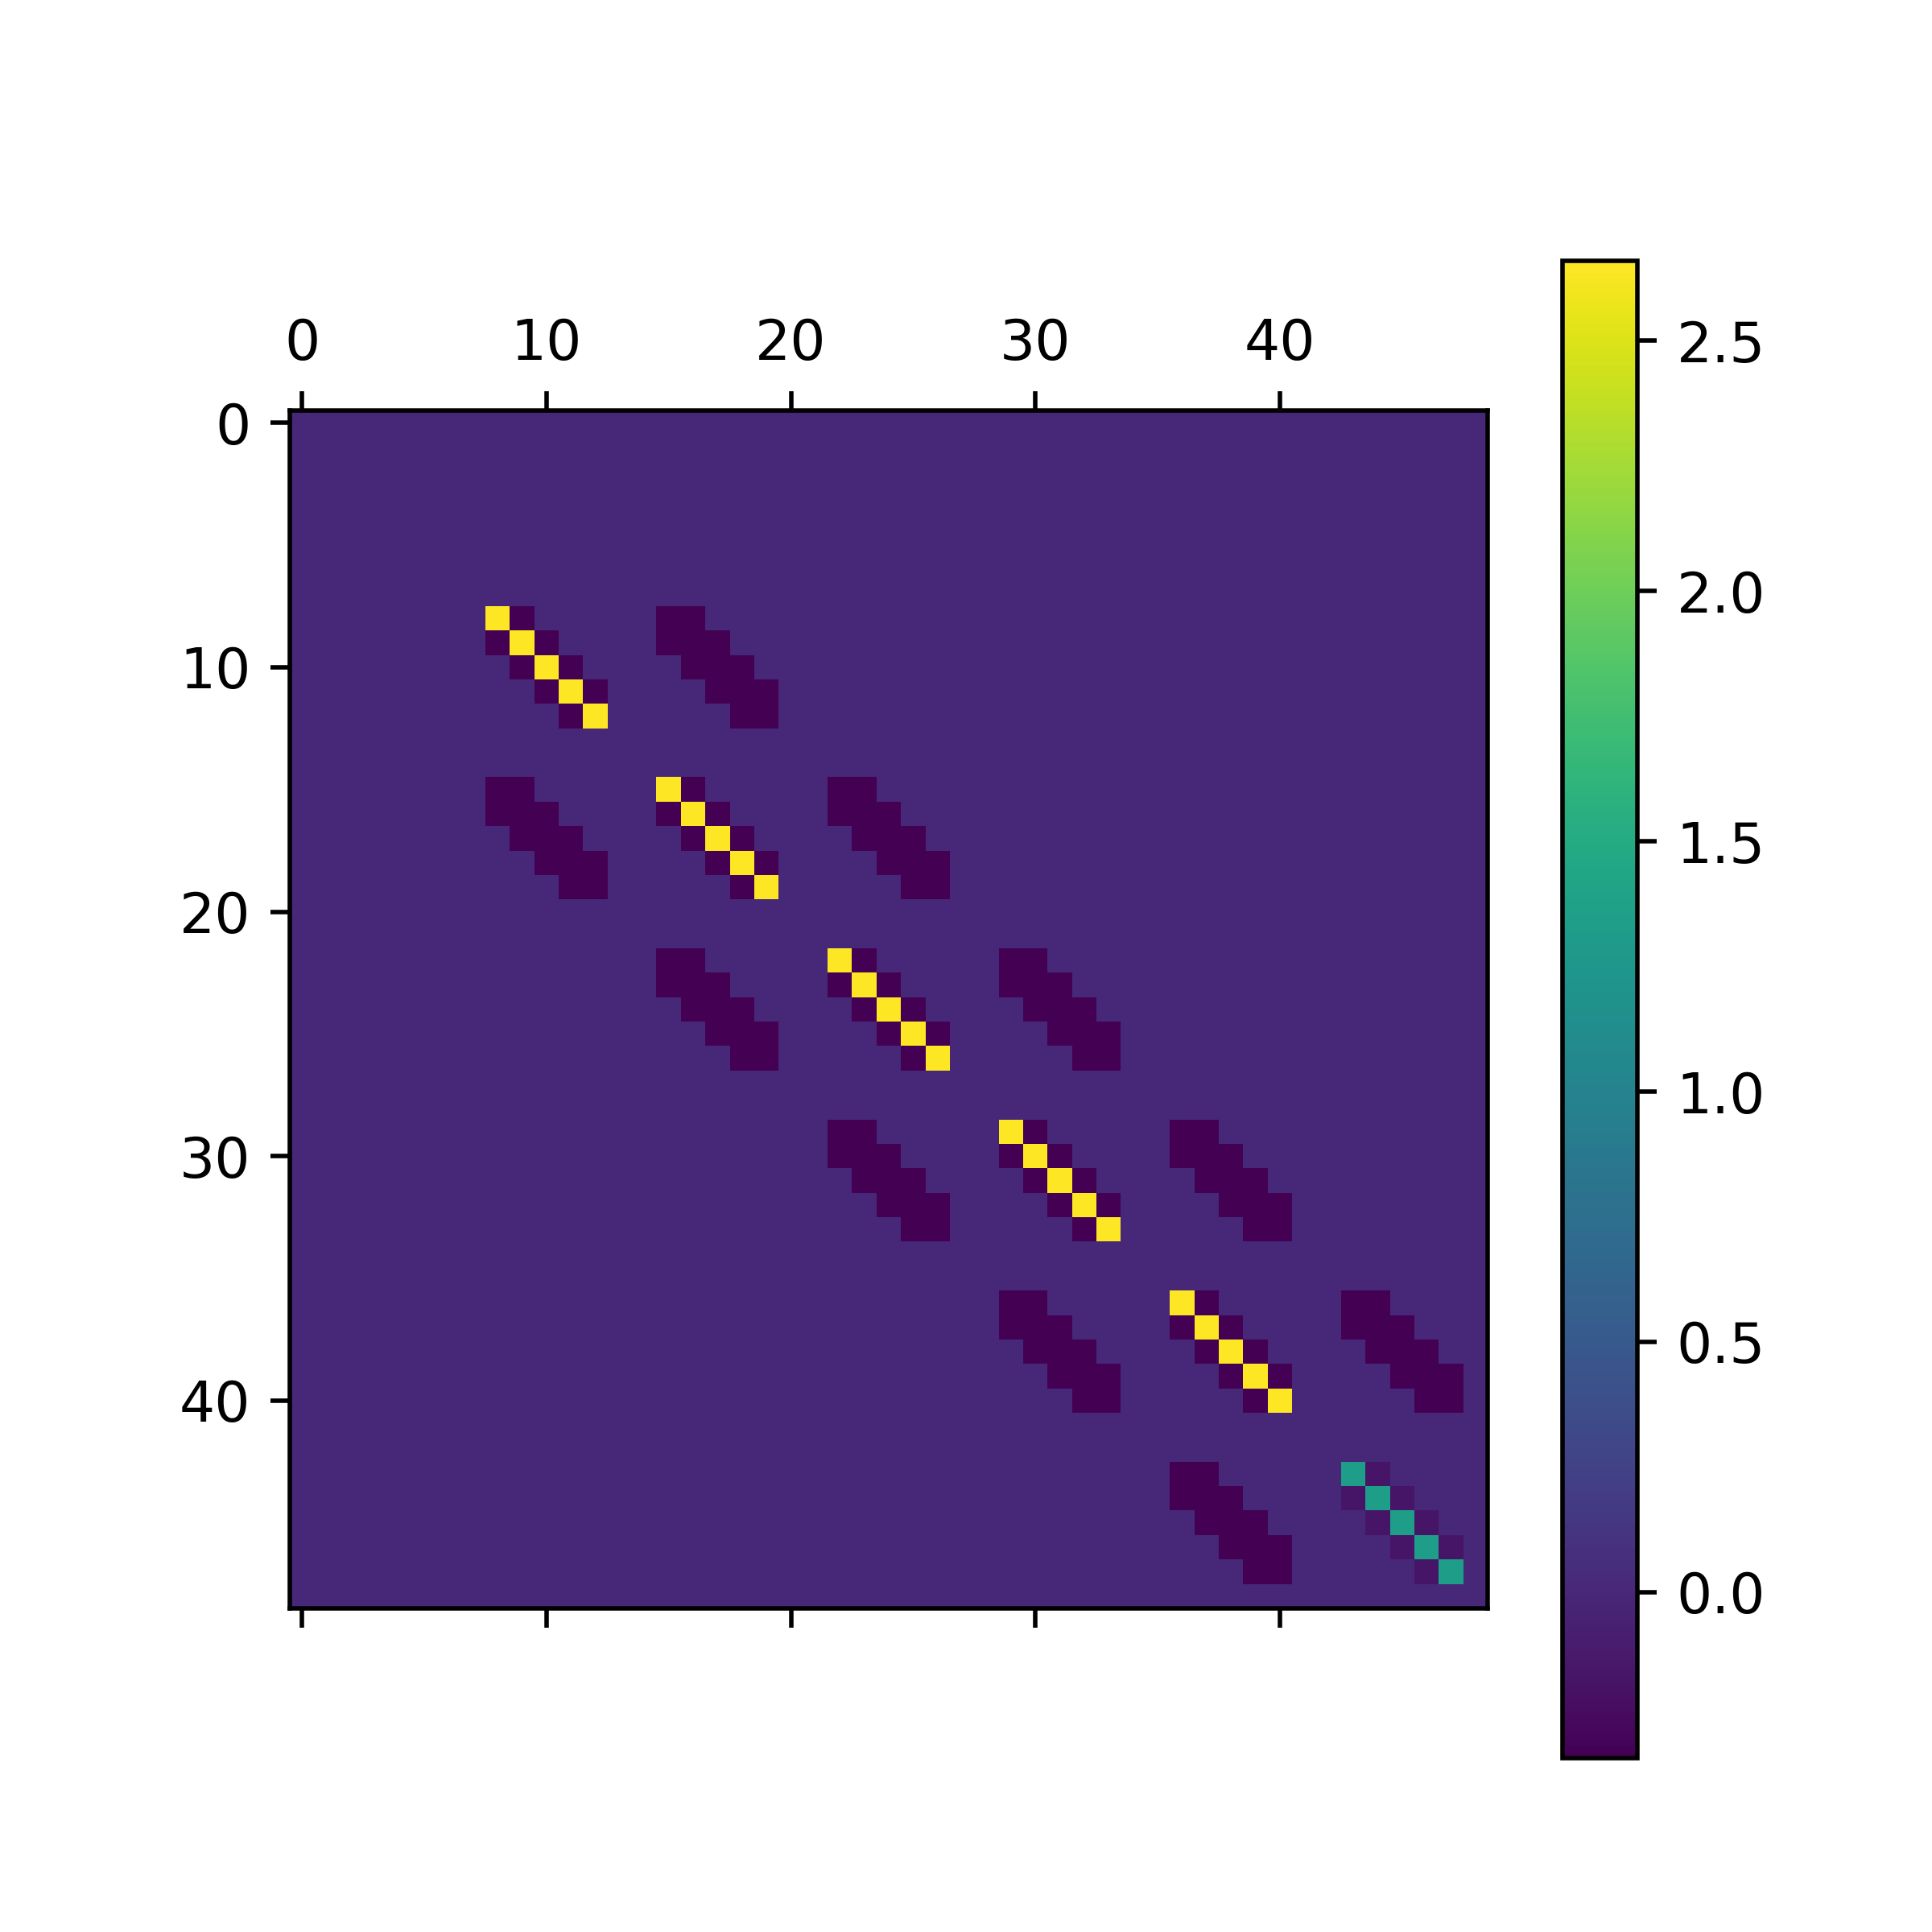
\includegraphics[width=9cm]{poisson 2d/(Poisson_2d)_(mat)_(neumann)_(vertex_num_49).png}
    \caption{Matrix A for 49 nodal points}
    \label{fig:basis}
\end{figure}
\\
\\
Observe below the two dimensional plot of the solution $u$ to this problem with the forcing function $$f(x,y) = -2y.$$ 
\begin{figure}[hbt!]
    \centering
    \includegraphics[width=10cm, , height=8cm]{poisson 2d/(Poisson_2d)_(neumann)_(vertex_num_49) (1).png}
    \caption{Solution to $\nabla^{2}u = -2y$ with mixed boundary conditions}
    \label{fig:basis}
\end{figure}
\\
To verify that our numerical solution is correct, we would have to know the analytic solution to our PDE. Fortunately, the choice of this problem was derived from a chosen solution i.e. for the function $$u(x,y) = -yx(x-1)$$ we find a suitable $f(x,y)$ so that the equation \[\nabla^{2}u(x,y) = f(x,y)\] holds. Since the Laplacian of $-yx(x-1)$ is $-2y$, we obtain our required forcing function $$f(x,y) = -2y.$$ The solution $u$ also contains the information for the boundary conditions required for the problem. Plotting the predetermined analytic solution in Wolfram Alpha, we are able to see that our computationally derived solution is indeed correct. 
\\
\\ 
\subsection{Another Two Dimensional Poisson Problem}
Now that we have the necessary computational tools, we also decided to solve the two dimensional Poisson problem for the forcing function $$f(x,y) = - 2\pi^2\sin{(\pi x)}\sin{(\pi y)}$$
with only the Dirichlet boundary condition $$u(x,y) = 0 \, \textrm{on } \,\partial\Omega. $$ The results we obtain for the matrix $A$ and the solution $u(x,y)$ are seen below.
\begin{figure}[hbt!]
\centering
\begin{minipage}{.5\textwidth}
    \centering
    \includegraphics[width=8cm]{poisson 2d/(Poisson_2d)_(mat_A)_(vertex_num_49) (1).png}
    \caption{Matrix A for 49 nodal points}
    \label{fig:Solution}

\end{minipage}%
\begin{minipage}{.5\textwidth}
    \centering
    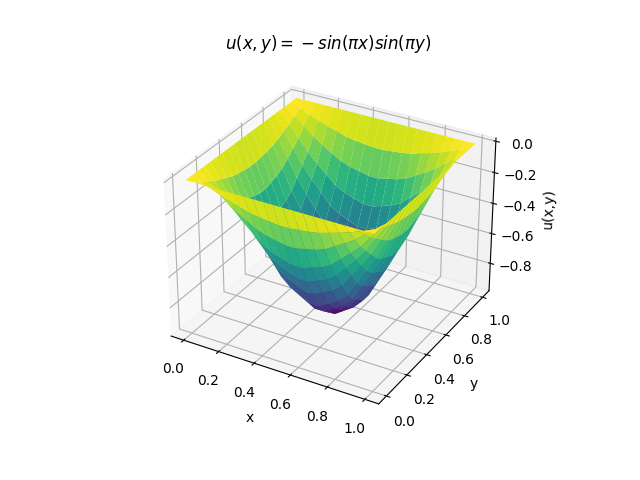
\includegraphics[width=8cm, height=7.5cm ]{poisson 2d/(Poisson_2d)_(vertex_num_49).png}
    \caption{Solution for 49 nodal points}
    \label{fig:Solution}

\end{minipage}
\end{figure}

\section{Heat Equation}
The heat equation is a fundamental partial differential equation in both pure and applied mathematics. It describes the diffusion of a property such as heat in a given domain over some time $t$. Here we aim to solve the following form of the heat equation:
$$\frac{\partial u}{\partial t} = \nabla^2u + f$$
where $u = u(x,y,t)$ is a function of two spacial variables and one time variable. For this problem we let the spacial domain be the unit square $[0,1]\times[0,1]$ and impose the usual Dirichlet boundary conditions
$$u(x,y,t) = 0 \quad \textrm{on } \,\partial\Omega. $$
We additionally impose initial conditions
$$u(x,y,0) = \sin{(\pi x)}\sin{(\pi y)}.$$
\subsection{Discretisation of Time}



\section{Stokes Equation}
\section{Non-Linear Poisson Problem}
We also decided to study a non-linear differential equation. As a continuation of our investigation into Poisson problems, we chose the non-linear Poisson Equation  $$-\nabla \cdot((u+1)\nabla u) = f.$$
































\section{References}
Note that certain books/articles may be written under one heading of references, but used throughout all the sections.
Background:
\begin{itemize}
\item https://doi.org/10.1590/1806-9126-RBEF-2017-0239
\item https://www.claymath.org/millennium/navier-stokes-equation/
\end{itemize}
Computational Methods:
\begin{itemize}
\item https://doi.org/10.1016/B978-1-4557-3141-1.50031-9
\item https://doi.org/10.1016/B978-0-12-824117-2.00011-9
\item https://doi.org/10.1016/B978-0-12-815601-8.50006-9
\end{itemize}
One Dimensional Poisson Problem:
\begin{itemize}
\item https://www.youtube.com/watch?v=P4lBRuY7pC4
\item https://jsdokken.com/dolfinx-tutorial/chapter1/fundamentals.html
\item Johnson, C. (n.d.). Numerical solution of partial differential equations by the finite element method. Courier Corporation.
\end{itemize}
Two Dimensional Poisson Problem:
\begin{itemize}
\item https://mathworld.wolfram.com/L2-Space.html
\item https://www.math.uci.edu/~chenlong/226/Ch2FEM.pdf
\item\href{https://fenicsproject.org/pub/tutorial/sphinx1/._ftut1003.html}{https://fenicsproject.org/pub/tutorial/sphinx1/.ftut1003.html}
\end{itemize}
Non Linear Poisson Problem:
\begin{itemize}
\item https://jsdokken.com/dolfinx-tutorial/chapter2/nonlinpoisson.html
\end{itemize}
Heat Equation:
\begin{itemize}
\item 
\end{itemize}


\end{document}


 